%% ----------------------------------------------------------------
%% Thesis.tex -- MAIN FILE (the one that you compile with LaTeX)
%% ----------------------------------------------------------------

% Set up the document
% Use the "Thesis" style, based on the ECS Thesis style by Steve Gunn
\documentclass[a4paper, 11pt, oneside]{Thesis}
% Location of the graphics files (set up for graphics to be in PDF format)
\graphicspath{{Figures/}}

% Include any extra LaTeX packages required
% Use the "Natbib" style for the references in the Bibliography
\usepackage[square, numbers, comma, sort&compress]{natbib}
% Needed for the "comment" environment to make LaTeX comments
\usepackage{verbatim}
% Allows "\bvec{}" and "\buvec{}" for "blackboard" style bold vectors in maths
\usepackage{vector}
% Colours hyperlinks in blue, but this can be distracting if there are many
% links.
\hypersetup{urlcolor=blue, colorlinks=true}

%% ----------------------------------------------------------------
\begin{document}
% Begin Roman style (i, ii, iii, iv...) page numbering
\frontmatter

% Set up the Title Page
\title  {Skill Social Network} \authors  {\texorpdfstring
{\href{dima@ceata.org}{Dumitru Ursu}} {Dumitru Ursu} }
% Do not change this here, instead these must be set in the "Thesis.cls" file,
% please look through it instead
\addresses  {\groupname\\\deptname\\\univname} \date       {\today} \subject
{} \keywords   {}

\maketitle
%% ----------------------------------------------------------------
% It is better to have smaller font and larger line spacing than the other way
% round
\setstretch{1.3}

% Define the page headers using the FancyHdr package and set up for one-sided
% printing
\fancyhead{}  % Clears all page headers and footers \rhead{\thepage}  % Sets the
right side header to show the page number \lhead{}  % Clears the left side page
header

 % Finally, use the "fancy" page style to implement the FancyHdr headers
\pagestyle{fancy}

%% ----------------------------------------------------------------
% Declaration Page required for the Thesis, your institution may give you a
% different text to place here
\Declaration{

\addtocontents{toc}{\vspace{1em}}  % Add a gap in the Contents, for aesthetics

I, Dumitru Ursu, declare that this thesis titled, `Skill social network' and the
work presented in it are my own. I confirm that:

\begin{itemize}
\item[\tiny{$\blacksquare$}] This work was done wholly or mainly
            while in candidature for a research degree at this University.

\item[\tiny{$\blacksquare$}] Where any part of this thesis has previously been
    submitted for a degree or any other qualification at this University or any
    other institution, this has been clearly stated.

\item[\tiny{$\blacksquare$}] Where I have consulted the published work of
    others, this is always clearly attributed.

\item[\tiny{$\blacksquare$}] Where I have quoted from the work of others, the
    source is always given. With the exception of such quotations, this thesis
    is entirely my own work.

\item[\tiny{$\blacksquare$}] I have acknowledged all main sources of help.

\item[\tiny{$\blacksquare$}] Where the thesis is based on work done by myself
jointly with others, I have made clear exactly what was done by others and what
I have contributed myself.  \\
\end{itemize}

Signed:\\ \rule[1em]{25em}{0.5pt}  % This prints a line for the signature

Date:\\ \rule[1em]{25em}{0.5pt}  % This prints a line to write the date
}
\clearpage  % Declaration ended, now start a new page

%% ----------------------------------------------------------------
% The "Funny Quote Page"
\pagestyle{empty}  % No headers or footers for the following pages

\null\vfill
% Now comes the "Funny Quote", written in italics
\textit{``Aut disce aut discede''}\\
\textit{``Either learn or go away''}


\begin{flushright} Latin saying \end{flushright}

\vfill\vfill\vfill\vfill\vfill\vfill\null
\clearpage  % Funny Quote page ended,
%% ----------------------------------------------------------------

% The Abstract Page
\addtotoc{Abstract} % Add the "Abstract" page entry to the Contents
\abstract{
\addtocontents{toc}{\vspace{1em}} % Add a gap in the Contents, for aesthetics

This thesis covers the design and implementation of a peer-to-peer teaching
network. The primary goals is to use cutting-edge technology in order to create
the social network and to explore unconventional virtual learning techniques.
One of the secondary goals of the system is to make it standard-based, web-only,
and so to make it accessible, and independent of proprietary technology.

In order to make the software more useful, it is released under a Free Software
license, \href{http://www.gnu.org/licenses/agpl-3.0.html}{AGPLv3}. The code can
be downloaded from \href{https://gitorious.org/discite/discite/}{Gitorious}, and
used without restrictions by universities or high schools. Deployment scripts
are provided, and so is documentation.

An instance of the application is running at \url{http://discite.info}. The
name of the application, "Discite", means "to learn" in Latin.

}

\clearpage  % Abstract ended, start a new page
%% ----------------------------------------------------------------

% Reset the line-spacing to 1.3 for body text (if it has changed)
\setstretch{1.3}

% The Acknowledgements page, for thanking everyone
\acknowledgements{
\addtocontents{toc}{\vspace{1em}}  % Add a gap in the Contents, for aesthetics

The acknowledgements and the people to thank go here, don't forget to include
your project advisor\ldots

}
\clearpage  % End of the Acknowledgements
%% ----------------------------------------------------------------

% The page style headers have been "empty" all this time, now use the "fancy"
% headers as defined before to bring them back
\pagestyle{fancy}


%% ----------------------------------------------------------------
\lhead{\emph{Contents}}  % Set the left side page header to "Contents"
\tableofcontents  % Write out the Table of Contents

%% ----------------------------------------------------------------
% Set the left side page header to "List if Figures"
\lhead{\emph{List of Figures}}
\listoffigures  % Write out the List of Figures

%% ----------------------------------------------------------------
% Set the left side page header to "List of Tables"
\lhead{\emph{List of Tables}}
\listoftables  % Write out the List of Tables

%% ----------------------------------------------------------------
\setstretch{1.5}  % Set the line spacing to 1.5, this makes the following tables easier to read
\clearpage  % Start a new page
\lhead{\emph{Abbreviations}}  % Set the left side page header to "Abbreviations"
\listofsymbols{ll}  % Include a list of Abbreviations (a table of two columns)
{
% \textbf{Acronym} & \textbf{W}hat (it) \textbf{S}tands \textbf{F}or \\
    \textbf{RoR} & \textbf{R}uby \textbf{o}n \textbf{R}ails \\
    \textbf{TDD} & \textbf{T}est \textbf{D}riven \textbf{D}evelopment\\
}

%% ----------------------------------------------------------------
% End of the pre-able, contents and lists of things
% Begin the Dedication page

\setstretch{1.3}  % Return the line spacing back to 1.3

\pagestyle{empty}  % Page style needs to be empty for this page
\dedicatory{For/Dedicated to/To my\ldots}

\addtocontents{toc}{\vspace{2em}}  % Add a gap in the Contents, for aesthetics


%% ----------------------------------------------------------------
\mainmatter % Begin normal, numeric (1,2,3...) page numbering
\pagestyle{fancy}  % Return the page headers back to the "fancy" style

% Include the chapters of the thesis, as separate files
% Just uncomment the lines as you write the chapters

% Chapter 1

\chapter{Introduction}
\label{Chapter1}
\lhead{Chapter 1. \emph{Introduction}}

\section{About}
``Discite'' is a web application for interactive peer-to-peer
teaching. As in mating sites, one can pick a teacher or a student based on
his/her interests, ratings and rankings, skills one is looking for, language of
teaching. The peer-to-peer process of learning allows screen sharing, video and
voice chat, presentations and doodling.

The web application belongs to the MOOC domain (Massive Open Online Course),
which is a novel approach to distance education.
The project is similar to several existing projects:
Coursera (\href{https://coursera.org}{\texttt{https://coursera.org}}),
Prezi (\href{https://prezi.com}{\texttt{https://prezi.com}}),
iversity (\href{htpps://iversity.org}{\texttt{https://iversity.org}}),
udacity (\href{https://udacity.com}{\texttt{https://udacity.com}})

What these systems are lacking is interactivity: most of them are just a site
hosting videos, tasks, and a forum for students.

The interactivity that ``Discite'' brings is some of life proved teaching
techniques, where a student can interrupt and change the way a lesson goes.
Teacher and students can alter the way a course goes, they can interact by chat,
doodling.
On the down side, the teacher and students have to meet at a certain time. The
course recordings can be watched after that, but that wont bring the
aforementioned benefits.

I think that as the time goes, more and more of the courses will be taken
online, and my application will fill a gap of teacher-student interaction
through the Internet.
Also, a useful feature is that not only teachers can create courses
(there is no concept of a teacher at the application level, there are just
course
owners), and anyone can see what teaching implies, and spread their skills to a
wide audience.

\section{Planning}
Objectives:\\
Provide an web-based implementation of a new way to have peer-to-peer lessons,
using open standards, based on cutting-edge technology.
Methodologies\\
Test Driven Development - is a approach to software development where you write
tests first, which fail, as no code can yet be run to fulfill
the test conditions. Then we write the minimal amount of code to make it pass,
and then we refactor the code if needed.
The upside of this approach is that the project doesn't go wild: the focus is
kept on the necessary features. Also, as we refactor the application
the test suite immediately shows if our changes broke the functionality in other
parts of the application.
The downside: we write as much test code as actual code that will be run. But
the experience shows us that it pays off in the long term.\\
Technologies:
\begin{itemize}
    \item Ruby - ``A dynamic, open source programming language with a focus on
        simplicity and productivity.
        It has an elegant syntax that is natural to read and easy to write.''
        \href{https://wwww.ruby-lang.org/en/}{\texttt{www.ruby-lang.org/en}}
    \item \href{http://rubyonrails.org}{\texttt{Ruby on Rails}} - a MVC
        (Model-View-Controller) server-side web development framework, backed by
        the Ruby language
    \item \href{http://foundation.zurb.com/}{\texttt{Zurb Foundation}} - A
        responsive front-end framework
    \item \href{https://github.com/plataformatec/devise}{\texttt{Devise}} for
        authentication
    \item \href{http://www.webrtc.org/}{\texttt{WebRTC}} Real-Time Communication
        implemented in browser, with a simple JavaScript API
\end{itemize}
I choose these technologies as I already have experience with most of them. The
one that I'm not familiar with is WebRTC:
it's a very young project, aiming to enable creation of rich web applications
with HTML5. It's still a
\href{http://dev.w3.org/2011/webrtc/editor/webrtc.html}{\texttt{draft}} at W3C
Nonetheless, the technology is already implemented in 2 popular browser: Google
Chrome and Mozilla Firefox.
Features:
\begin{itemize}
    \item pick a course based on your interests
    \item give the course and teacher a rating
    \item choose a preferred language
    \item filter by skills one is looking for
    \item screen sharing
    \item voice/video chat
    \item presentation
    \item doodling
\end{itemize}
Technical challenges - screen sharing, audio/video chat is very
compute-intensive operation, and while the connections are peer-to-peer
a user will a older computer would not be able to handle the decoding of tens of
videos. This is why a limitation must be introduced in the
application: only the teacher can broadcast/share his screen and video/audio
chat. Presentations - HTTP, the protocol used for web page delivery
on the web, is a stateless protocol. Presentations have to be stateful, so
teacher and students will see the same slide at the same time.
Add a citing by \citet{tenderlove} tender love.
 % Introduction

% Chapter 2

\chapter{Methods Used}
\label{Chapter2}
\lhead{Chapter 2. \emph{Methods Used}}

\section{Test-Driven Development}
Test-Driven Development is a software development methodology and strategy that
requires test to written first (the red stage), then write just enough code to
make the tests pass (the green stage), and the analyze the code written, and
change it if necessary (the refactor stage). By necessity we mean either changing
the code for performance reasons, readability, consistency with the rest of the
codebase, or other reasons.
\subsection{Page-Objects}
 % Methods Used

% Chapter 3

\chapter{User Testing}
\label{Chapter3}
\lhead{Chapter 3. \emph{User Testing}}

 % User testing

% Chapter 4

\chapter{Conclusions}
\label{Chapter4}
\lhead{Chapter 4. \emph{Conclusions}}

 % Conclusions


%% ----------------------------------------------------------------
% Now begin the Appendices, including them as separate files

\addtocontents{toc}{\vspace{2em}} % Add a gap in the Contents, for aesthetics

\appendix % Cue to tell LaTeX that the following 'chapters' are Appendices

% Appendix A

\chapter{User's Manual}
\label{AppendixA}
\lhead{Appendix A. \emph{User's Manual}}

Write your Appendix content here.
 % User's Manual

% Appendix B

\chapter{Maintenace Manual}
\label{AppendixB}
\lhead{Appendix B. \emph{Maintenance Manual}}

Write your Appendix content here.
 % Maintenance Manual

% Appendix C

\chapter{Design Documents}
\label{AppendixC}
\lhead{Appendix C. \emph{Design Documents}}

\begin{figure}[htbp]
\centering
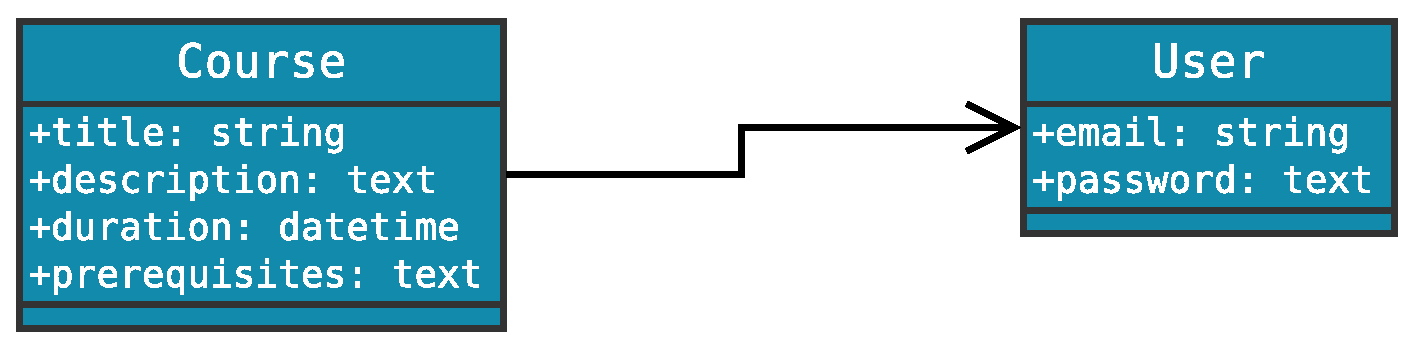
\includegraphics{./Figures/discite.eps}
\rule{35em}{0.5pt}
\caption[An Electron]{An electron (artist’s impression).}
\label{fig:Electron}
\end{figure}
 % Design Documents

% Appendix D

\chapter{Source Code}
\label{AppendixD}
\lhead{Appendix D. \emph{Source Code}}

Write your Appendix content here.
 % Source Code

% Appendix E

\chapter{Test Suite}
\label{AppendixD}
\lhead{Appendix D. \emph{Test Suite}}

% let's define some commands to include the test suite
\newcommand{\lTest[1]}{\lstinputlisting[style=ruby]{/home/dimon/sandbox/rails/discite/spec/\string#1}}
\newcommand{\lFeatureTests[1]}{\lstinputlisting[style=ruby]{/home/dimon/sandbox/rails/discite/spec/features/\string#1}}
\newcommand{\lPagesTests[1]}{\lstinputlisting[style=ruby]{/home/dimon/sandbox/rails/discite/spec/pages/\string#1}}


\lTest[spec_helper.rb]

\lFeatureTests[home_spec.rb]

\lPagesTests[home_page.rb]
 % Test Suite

\addtocontents{toc}{\vspace{2em}}  % Add a gap in the Contents, for aesthetics
\backmatter

%% ----------------------------------------------------------------
\label{Bibliography}
% Change the left side page header to "Bibliography"
\lhead{\emph{Bibliography}}
% Use the "unsrtnat" BibTeX style for formatting the Bibliography
\bibliographystyle{unsrtnat}
% The references (bibliography) information are stored in the file named
% "Bibliography.bib"
\bibliography{Bibliography}

\end{document}  % The End
%% ----------------------------------------------------------------
